\documentclass{standalone}
\usepackage{tikz}
\usepackage{tkz-euclide}
\usepackage{ctex}
\pagestyle{empty}
\setCJKmainfont{Noto Serif CJK SC}
\usepackage{siunitx,chemmacros,chemfig}
\setchemfig{bond offset = 0pt}
\chemsetup[orbital]{
  overlay,
  opacity=0.5,
  sp/scale=2.5,
  p/scale=2.5,
  s/color=blue!50,
  s/scale=1.8
}
\begin{document}
\small
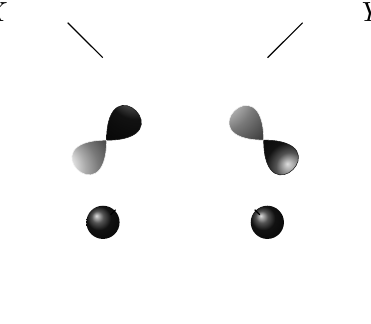
\begin{tikzpicture}
  \useasboundingbox(-2.0,-1.7)rectangle(2.0,1.7);
  % \draw[very thin](0,0)--(45:1.5)(0,0)--(-45:1.5);
  \node(a) {
  \chemfig{
    \orbital{s}-[:45,1.4]{\orbital[angle=45]{p}}
    {\orbital[angle=-45]{p}}
    % {\orbital[angle=210]{sp}}
    % {\orbital[angle=240]{sp}}
    (-[:45,2.0])(-[:135,2.0])
    -[:-45,1.4]\orbital{s}
    }
  };
\node at (a.north east)[right]{$Y$};
\node at (a.north west)[left]{$X$};
\end{tikzpicture}
\end{document}